% test.tex
\title{Housing Analysis in Austria based on Demographic Evolution}
\author{Dominik Lindorfer (\href{mailto:dlindo@posteo.at}{dlindo@posteo.at})}

\newcommand{\abstractText}{\noindent
Throughout the past 10 years housing prices have increased significantly in Austria. This analysis uses demographic data of Austrians to explain this increase and to predict the price-trend for the next period from 2021 - 2040. Potential buyers of houses can possibly use this information to avoid purchasing their new home at an excess price.
}

%%%%%%%%%%%%%%%%%
% Configuration %
%%%%%%%%%%%%%%%%%

\documentclass[11pt, a4paper, twocolumn]{article}
\usepackage{xurl}
\usepackage[super,comma,sort&compress]{natbib}
\usepackage{abstract}
\renewcommand{\abstractnamefont}{\normalfont\bfseries}
\renewcommand{\abstracttextfont}{\normalfont\small}

\usepackage{geometry}
\geometry{top=1cm,bottom=1.5cm,left=1.5cm,right=1.5cm,includefoot}
\setlength{\columnsep}{7mm} % Column separation width
\usepackage{graphicx}
\usepackage[labelfont=bf]{caption}
\usepackage{float}
%%%%%%%%%%%%%%
% References %
%%%%%%%%%%%%%%

% If changing the name of the bib file, change \bibliography{test} at the bottom
\begin{filecontents}{test.bib}

@misc{LinkReference1,
  title        = "Link Title",
  author       = "Link Creator(s)",
  howpublished = "\url{https://example.com/}",
}

@misc{Author1,
  author       = "LastName, FirstName",
  howpublished = "\url{mailto:email@example.com}",
}

@article{ArticleReference1,
  author  = "Lastname1, Firstname1 and Lastname2, Firstname2",
  title   = "Article title",
  year    = "Year",
  journal = "Journal name",
  note    = "\url{https://dx.doi.org/...}",
}

\end{filecontents}

% Any configuration that should be done before the end of the preamble:
\usepackage{hyperref}
\hypersetup{colorlinks=true, urlcolor=blue, linkcolor=blue, citecolor=blue}

\begin{document}

%%%%%%%%%%%%
% Abstract %
%%%%%%%%%%%%

\twocolumn[
  \begin{@twocolumnfalse}
    \maketitle
    \begin{abstract}
      \abstractText
      \newline
      \newline
    \end{abstract}
  \end{@twocolumnfalse}
]

%%%%%%%%%%%
% Article %
%%%%%%%%%%%

\section{Introduction\label{ch:Introduction}}

Most young families in Austria today are confronted with seemingly every increasing housing prices during their adult life. This paper tries to predict the price-trend for the future period 2021 - 2040 to help with the common question: "should we buy a new home now or wait"? To do so, demographic data of Austrians is used to categorize people into potential home buyers and potential home sellers by using their age and it is shown that the number of people in these groups starts to diverge after the year 2020, indicating the start of a buyers market. Furthermore several difficulties and possible extensions to this analysis are discussed.
\vspace{0.2cm}

\begin{figure}[!ht]
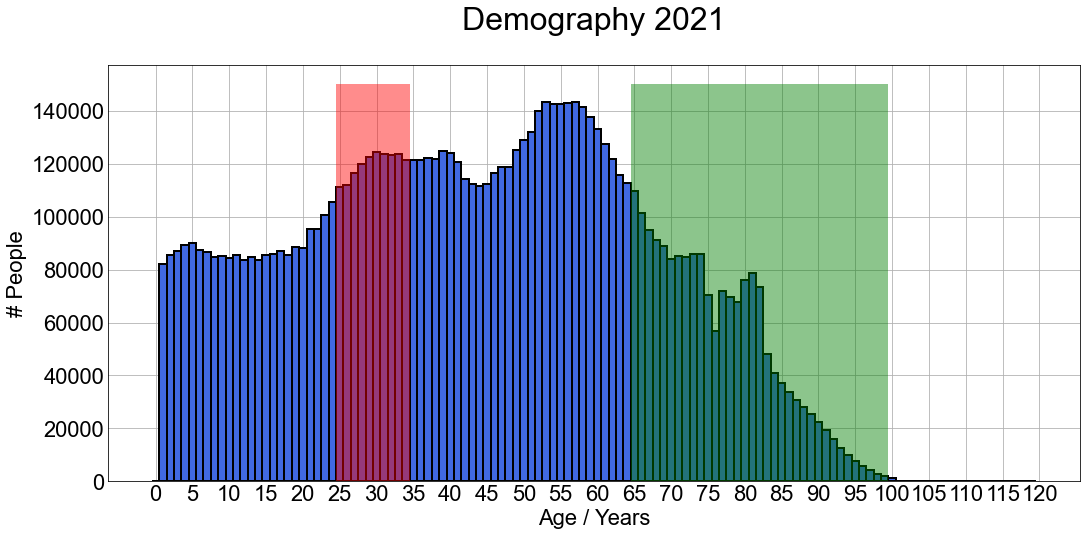
\includegraphics[width=0.45\textwidth]{../Figures/Demog2021.png}
\caption{\small Demography in Austria today at the end of 2021. Two distinct peaks in the bar-chart show at age 50-60 years show the baby-boomers of the 1960s and their children between the age of 25-40 years. The red and green rectangles show the home-buyer and home-seller sub-groups. \label{Demog2021}}
\end{figure}

\section{Data}

Demographic data has been obtained from Statistik Austria [1] for the years 2004 to 2021. The demography has been divided into sub-groups of people between 25-35 years (potential home buyers) and people between 65-100 years (potential home sellers). To forecast the demographic evolution between 2021 to 2040 the demographic data has been shifted linearly for each year, respectively, e.g. the number of people that are 25 years in 2021 old will be forecast to be 30 years old in 2026. To account for mortality in the 65-100 group, a mean mortality of 70000 per year has been calculated for the years 2004 to 2021. Thus, the total number of people in the 65-100 group is then reduced by 70000 for each year from 2021 - 2040 in the forecast.


\section{Results}

\subsection*{Demography Today and Forecast}
The demography in Austria today (end of 2021) indicates two very distinct peaks when drawn as a bar-chart (Fig. \ref{Demog2021}): the right most peak between the age 50-60 years is due to the baby boom in the 1960s and their children, who are now mainly between the age of 25-40 years old, account for the second peak to the left. The red and green rectangles show the home-buyer and home-seller sub-groups.

By linearly shifting the demography along the age axis, a forecast of the population for the coming years can be estimated. In Fig. \ref{Demog_Forecast} the demographic evolution from 2004 to 2040 is shown, where the years 2004-2021 use data from Statistik Austria (see above) and the years 2022-2040 use forecast data. The red and green boxes mark the age-groups 25-35 years (potential home buyers) and people between 65-100 years (potential home sellers), respectively. It can be seen, that the number of people in the red rectangle decreases from 2020 forward to 2040 while the number of people within the green rectangle increases. In Fig. \ref{Buyer_Seller} the total numbers of home-buyers and home-sellers is shown as blue and red curves, respectively. Please note that the idea behind this segmentation is, that people between 25-35 years are often starting a family and are thus more likely to buy a new home while people between age 65-100 years are more likely to sell their existing house or flat due to their children no longer living with them or, in general, the desire to spend less time in a large living space.

\begin{figure}[!ht]
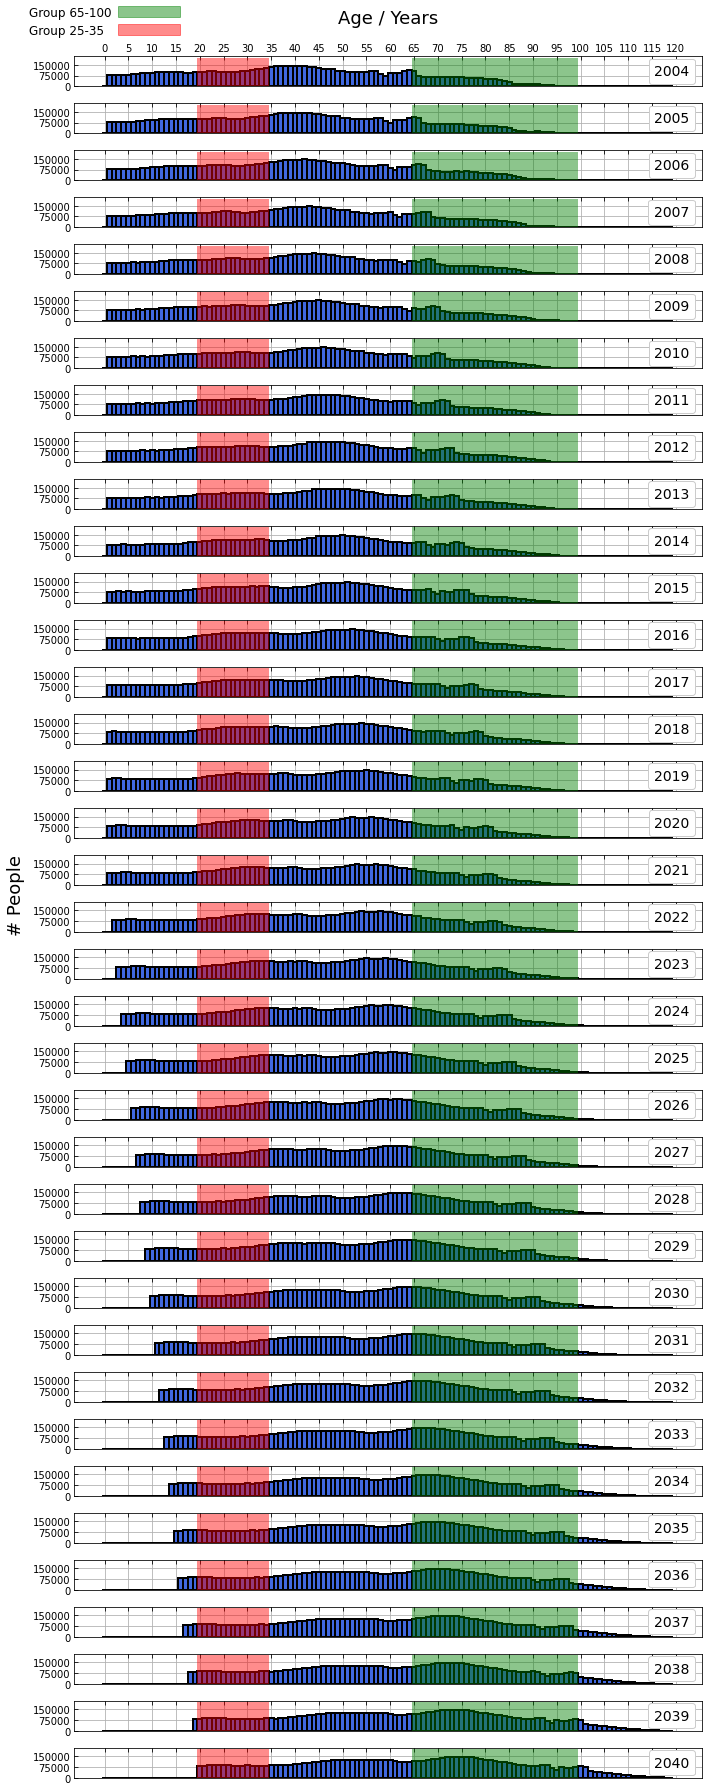
\includegraphics[width=0.49\textwidth]{../Figures/Demog_Forecast.png}
\caption{\small Demographic evolution in Austria from 2004 to 2040. The years 2004-2021 use data from Statistik Austria (see above) and the years 2022-2040 use forecast data. The red and green boxes mark the age-groups 25-35 years (potential home buyers) and people between 65-100 years (potential home sellers). \label{Demog_Forecast}}
\end{figure}

\subsection*{Why did Housing-Prices increase from 2008-2021?}

In Fig. \ref{Buyer_Seller} the total number of people in the buyer and seller sub groups are shown as blue and red curves. It is evident, that from 2004 until the housing crisis in 2008 the housing market was already starting to cool off. Still, there have been more potential home buyers than sellers in the period 2004 - 2020. In the period 2020-2040, however, this trend changes dramatically showing a wide spread between the number of buyers and sellers. This result is intuitive, as more and more people born during the baby boom era enter the age group between 65-100 while their children already have started their own families and no longer are looking for a new place to stay.

\begin{figure}[H]
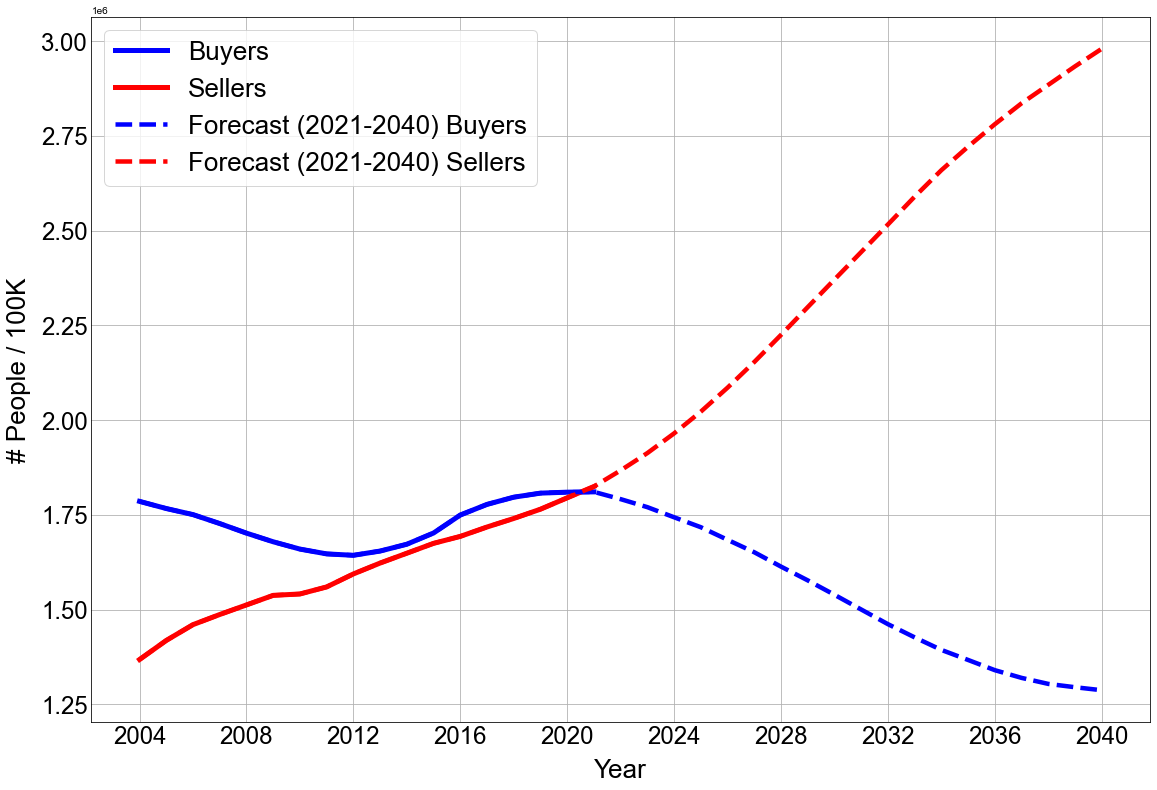
\includegraphics[width=0.45\textwidth]{../Figures/BS.png}
\caption{\small Total numbers of home-buyers (age-group 25-35 years) and home-sellers (age-group 65-100 years) using the demographic data (and forecast) from Fig. \ref{Demog_Forecast}. From year 2020 on it can be seen that there will be a large gap between those two groups. \label{Buyer_Seller}}
\end{figure}

\subsection*{When should I buy a new home?}
This analysis clearly suggests that there is a wide spread between potential home buyers and home sellers starting from 2020. In Fig. \ref{Buyer_Seller_Difference} the difference between the total number of sellers and buyers supports this result, suggesting that after 2020 there will be more people looking to sell than people looking to buy, thus entering a so-called buyers market. This view is supported further by forecasting the total number of houses and flats in Austria using the mean increase from 2005 to 2020 (Fig. \ref{Houses_Stock}). As a potential home buyer it is therefore better to wait several years (5+) in order to avoid paying an excess price and to give the market time to react to this new situation.

\begin{figure}[!ht]
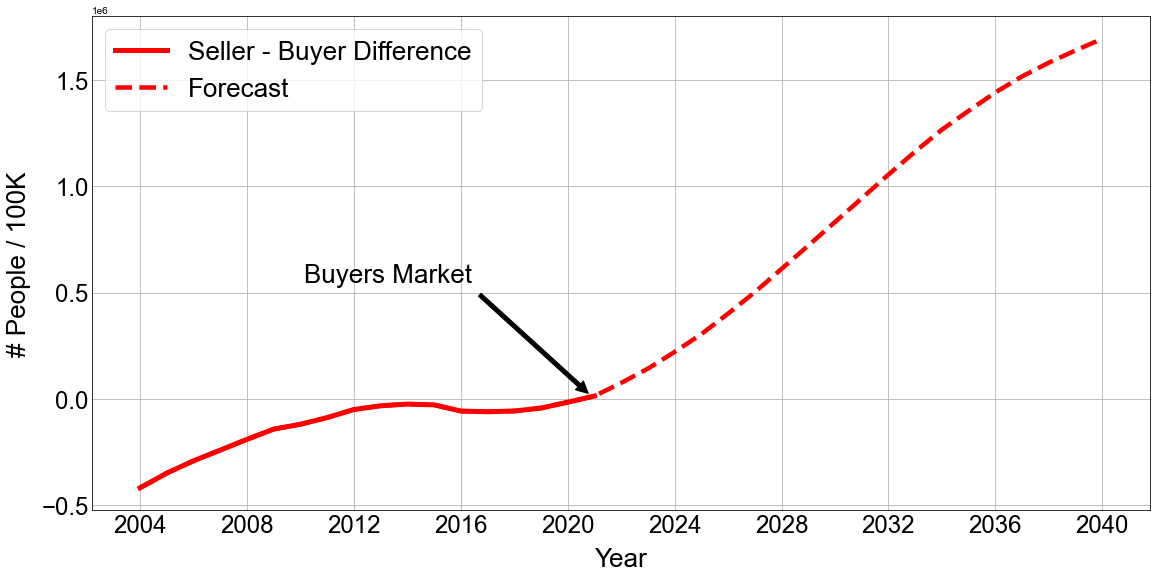
\includegraphics[width=0.45\textwidth]{../Figures/BS_Diff.png}
\caption{Difference between number of home-buyers (age-group 25-35 years) and home-sellers (age-group 65-100 years) using data shown in Fig. \ref{Buyer_Seller}. Starting from year 2020 the demography suggests a so-called buyers market with more home sellers than buyers.\label{Buyer_Seller_Difference}}
\end{figure}

Please note that this analysis has several flaws, some of which are listed below with a prefix that might work in favor \color{green}{(pro)} \color{black} or in opposite \color{red}{(contra)} \color{black} to this conclusion

\begin{enumerate}
	\item \color{green}{(pro)} \color{black} Rising interest rates potentially make investments in real estate less attractive, thus increasing the amount of real estate on the market.
	\item \color{green}{(pro)} \color{black} Credit risk in Austria related to housing is finally recognized by state institutions \href{https://orf.at/stories/3247123/}{(Link)} and stricter tightening is considered for 2022.
	\item \color{red}{(contra)} \color{black} The housing market is often not rational, i.e. there might be a market stand-still or a wait and see.
	\item \color{red}{(contra)} \color{black} Due to the corona crisis, more people are happy to have large living spaces, although they do not necessarily need it (nice to have).
	\item \color{red}{(contra)} \color{black} It is not clear that the amount of houses increases at the current rate as forecast in Fig. \ref{Houses_Stock}.
\end{enumerate}

\begin{figure}[H]
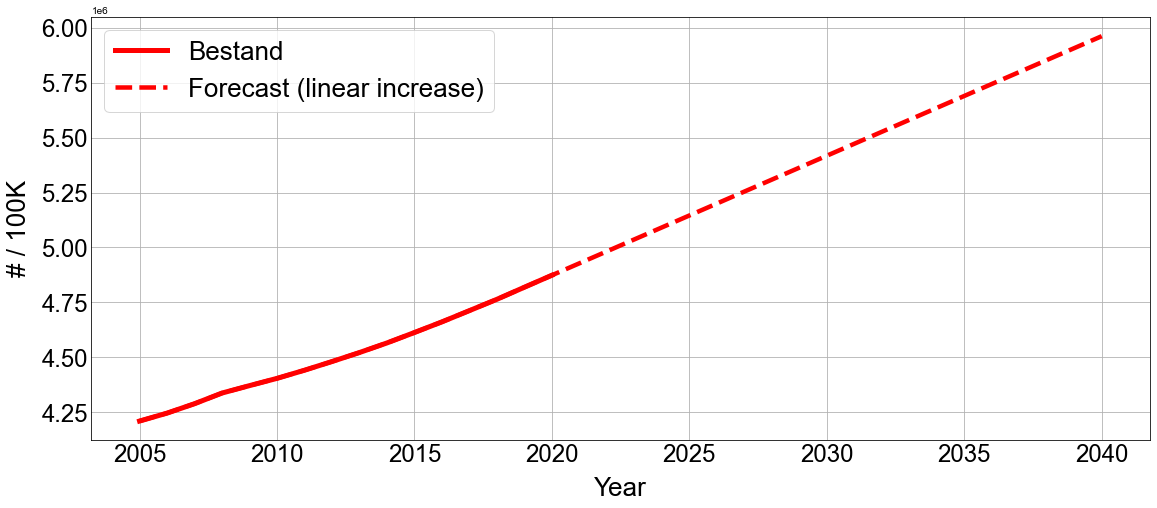
\includegraphics[width=0.45\textwidth]{../Figures/Bestand.png}
\caption{Total number of houses and flats in Austria and forecast using the mean increase from 2005 to 2020 \label{Houses_Stock}}
\end{figure}


%%%%%%%%%%%%%%
% References %
%%%%%%%%%%%%%%

\section*{References}

[1] Statistik Austria Stat. Database: \url{https://pic.statistik.at/web_de/statistiken/index.html}


\nocite{*}
\bibliographystyle{plain}
\bibliography{test}

\end{document}
